\documentclass[tikz]{standalone}
\usepackage[utf8]{inputenc}
\usetikzlibrary{calc,shadows}

\definecolor{mycolor}{RGB}{12,18,33}

\begin{document}
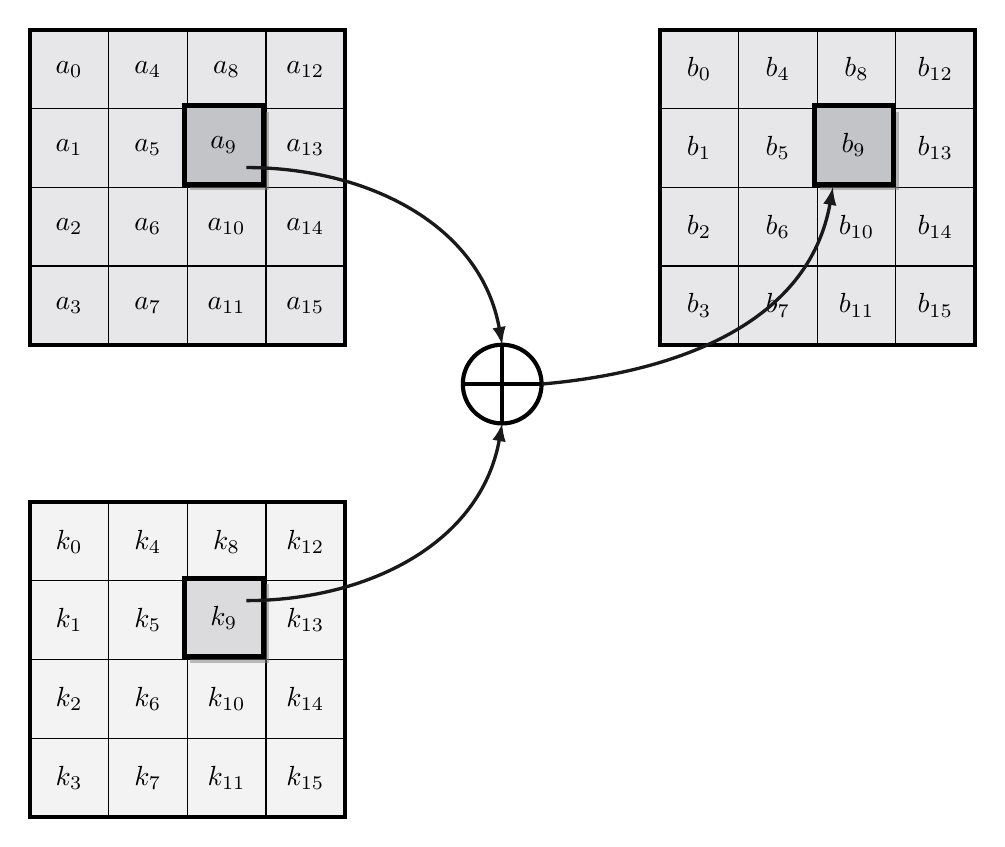
\begin{tikzpicture}
% state before
\foreach\x in {0, 1, ..., 3}
\foreach\y in {0, 1, ..., 3}
\draw[fill=mycolor!10] (\x,\y) rectangle ($(\x,\y) + (1,1)$);

\draw[line width=1.5pt] (0,0) rectangle (4,4);

\node at (0.5, 0.5) {$a_3$};
\node at (0.5, 1.5) {$a_2$};
\node at (0.5, 2.5) {$a_1$};
\node at (0.5, 3.5) {$a_0$};
\node at (1.5, 0.5) {$a_7$};
\node at (1.5, 1.5) {$a_6$};
\node at (1.5, 2.5) {$a_5$};
\node at (1.5, 3.5) {$a_4$};
\node at (2.5, 0.5) {$a_{11}$};
\node at (2.5, 1.5) {$a_{10}$};
\node at (2.5, 3.5) {$a_8$};
\node at (3.5, 0.5) {$a_{15}$};
\node at (3.5, 1.5) {$a_{14}$};
\node at (3.5, 2.5) {$a_{13}$};
\node at (3.5, 3.5) {$a_{12}$};

\draw[line width=1.8pt,drop shadow,shift={(-1pt,1pt)},fill=mycolor!25] (2,2) rectangle (3,3);
\node[shift={(-1pt,1pt)}] at (2.5, 2.5) {$a_9$};
\node (a) at (2.5,2.5) {};

% round key
\begin{scope}[shift={(0,-6)}]

\foreach\x in {0, 1, ..., 3}
\foreach\y in {0, 1, ..., 3}
\draw[fill=mycolor!5] (\x, \y) rectangle ($(\x, \y) + (1, 1)$);

\draw[line width=1.5pt] (0, 0) rectangle (4,4);

\node at (0.5, 0.5) {$k_3$};
\node at (0.5, 1.5) {$k_2$};
\node at (0.5, 2.5) {$k_1$};
\node at (0.5, 3.5) {$k_0$};
\node at (1.5, 0.5) {$k_7$};
\node at (1.5, 1.5) {$k_6$};
\node at (1.5, 2.5) {$k_5$};
\node at (1.5, 3.5) {$k_4$};
\node at (2.5, 0.5) {$k_{11}$};
\node at (2.5, 1.5) {$k_{10}$};
\node at (2.5, 3.5) {$k_8$};
\node at (3.5, 0.5) {$k_{15}$};
\node at (3.5, 1.5) {$k_{14}$};
\node at (3.5, 2.5) {$k_{13}$};
\node at (3.5, 3.5) {$k_{12}$};

\draw[line width=1.8pt,drop shadow,shift={(-1pt,1pt)},fill=mycolor!15] (2,2) rectangle (3,3);
\node[shift={(-1pt,1pt)}] at (2.5, 2.5) {$k_9$};
\node (k) at (2.5,2.5) {};
\end{scope}

% state after
\begin{scope}[shift={(8,0)}]

\foreach\x in {0, 1, ..., 3}
\foreach\y in {0, 1, ..., 3}
\draw[fill=mycolor!10] (\x, \y) rectangle ($(\x, \y) + (1, 1)$);

\draw[line width=1.5pt] (0, 0) rectangle (4,4);

\node at (0.5, 0.5) {$b_3$};
\node at (0.5, 1.5) {$b_2$};
\node at (0.5, 2.5) {$b_1$};
\node at (0.5, 3.5) {$b_0$};
\node at (1.5, 0.5) {$b_7$};
\node at (1.5, 1.5) {$b_6$};
\node at (1.5, 2.5) {$b_5$};
\node at (1.5, 3.5) {$b_4$};
\node at (2.5, 0.5) {$b_{11}$};
\node at (2.5, 1.5) {$b_{10}$};
\node at (2.5, 3.5) {$b_8$};
\node at (3.5, 0.5) {$b_{15}$};
\node at (3.5, 1.5) {$b_{14}$};
\node at (3.5, 2.5) {$b_{13}$};
\node at (3.5, 3.5) {$b_{12}$};

\draw[line width=1.8pt,drop shadow,shift={(-1pt,1pt)},fill=mycolor!25] (2,2) rectangle (3,3);
\node[shift={(-1pt,1pt)}] at (2.5, 2.5) {$b_9$};
\node (b) at (2.5,2.5) {};
\end{scope}

% big xor
\draw[line width=1.5pt] (6,-.5) circle (.5) node (xor) {};
\draw[line width=1.5pt] (5.5,-.5) -- (6.5,-.5);
\draw[line width=1.5pt] (6,-1) -- (6,0);

% arrows
\draw[-latex,line width=1.2pt,color=black!90] ($(a) + (.25,-.25)$) to[out=0, in=100] ($(6,-.5) + (90:.5)$);
\draw[-latex, line width=1.2pt,color=black!90] ($(k) + (.25,.25)$) to[out=0, in=-100] ($(6,-.5) + (-90:.5)$);
\draw[-latex, line width=1.2pt,color=black!90] ($(6,-.5) + (0:.5)$) to[out=5, in=-100] ($(b) + (-.3,-.5)$);
\end{tikzpicture}
\end{document}